\documentclass{standalone}
\usepackage{tkz-fct}
\usepackage{tkz-euclide}
\usepackage{color}
\renewcommand*\familydefault{\sfdefault}
\usepackage{sansmath}
\usepackage{amsmath}
\sansmath
\definecolor{gray75}{gray}{0.75}
\begin{document}
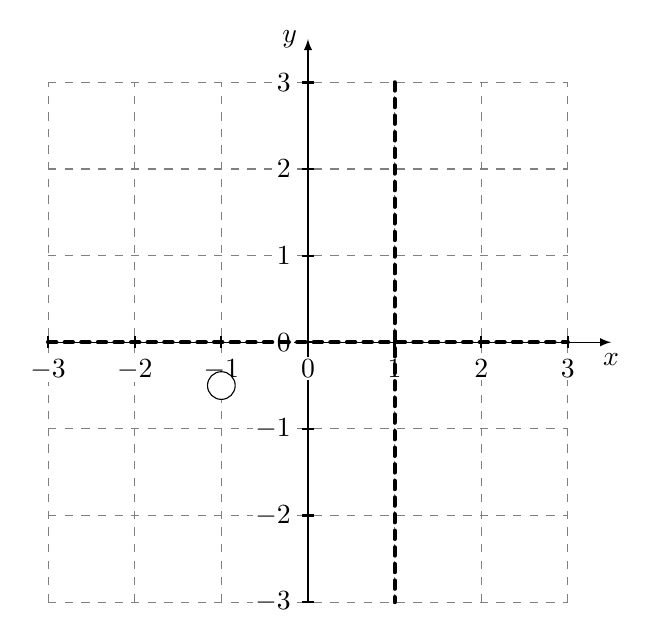
\begin{tikzpicture}[scale=1.1]
  \tkzInit[xmin=-3, xmax=3,ymin=-3,ymax=3]
  \begin{scope}[dashed]
    \tkzGrid
  \end{scope}
  \tkzDrawX[label={$x$}]
  \tkzDrawY[label={$y$}]
  \tkzLabelX
  \tkzLabelY
  \tkzFct[line width=2pt, domain=-3:0.7]{(x+1)/(x**2-1)}
  \tkzFct[line width=2pt, domain=1.3:3]{(x+1)/(x**2-1)}
  \tkzDefPoint(1,3){A}
  \tkzDefPoint(1,-3){B}
  \tkzDrawSegment[style=dashed,line width = 1.5pt](A,B)
  \tkzDefPoint(-3,0){A}
  \tkzDefPoint(3,0){B}
  \tkzDrawSegment[style=dashed,line width = 1.5pt](A,B)
  \tkzDrawPoint[size=10,color=black,fill=white](-1.0,-0.5)
\end{tikzpicture}
\end{document}
